\documentclass[fleqn]{article}
\usepackage{amsmath}
\usepackage{amsfonts} 
\usepackage{graphicx}
\usepackage{tabularx}

\begin{document}
\newcommand\tab[1][1cm]{\hspace*{#1}}
\section*{Numerical Optimization with Python -  Ex. 1: dry part}
Alon\\ \\



\underline{\textbf{Part 1}}:\\

\textbf{1.1} \\
Let $a \in \mathbb{R}^n, \; f:\mathbb{R}^n \rightarrow \mathbb{R}, \; f(x)=a^T x$ \\
Note: 
$f(x)=a^T x = \begin{pmatrix} a_1 & ... & a_n \\ \end{pmatrix}
\begin{pmatrix} x_1 \\ \vdots \\ x_n \\ \end{pmatrix} = 
 \sum_{i=1}^{n} a_i x_i 
$ \\ \\

a. \\
$
\nabla f(x) = \begin{bmatrix} \frac{\partial f}{\partial x_1} \\
				\vdots \\     \frac{\partial f}{\partial x_n} \\ \end{bmatrix} 
=
\begin{bmatrix} \frac{\partial \sum_{i=1}^{n} a_i x_i}{\partial x_1} \\
				\vdots \\     \frac{\partial \sum_{i=1}^{n} a_i x_i}{\partial x_n} \\ \end{bmatrix} 
=
\begin{bmatrix} a_1 \\ \vdots \\ a_n \\ \end{bmatrix} = a
$ \\ \\

b. \\
\[
\nabla^2 f(x) = \begin{bmatrix} 
\frac{\partial^2 f}{\partial x_1^2} & \frac{\partial^2 f}{\partial x_1 \partial x_2} & \cdots & \frac{\partial^2 f}{\partial x_1 \partial x_n}\
\\ 
\frac{\partial^2 f}{\partial x_1 \partial x_2} & \frac{\partial^2 f}{\partial x_2^2} & \cdots & \frac{\partial^2 f}{\partial x_2 \partial x_n}
\\ 
\vdots & \vdots & \ddots & \vdots
\\ 
\frac{\partial^2 f}{\partial x_1 \partial x_n} & \frac{\partial^2 f}{\partial x_2 \partial x_n} & \cdots & \frac{\partial^2 f}{\partial x_n^2}
\\ 
				\end{bmatrix}
=
\begin{bmatrix} 
\frac{a_1}{\partial x_1} & \frac{a_1}{\partial x_2} & \cdots & \frac{a_1}{\partial x_n}\
\\ 
\frac{a_2}{\partial x_1} & \frac{a_2}{\partial x_2} & \cdots & \frac{a_2}{\partial x_n}
\\ 
\vdots & \vdots & \ddots & \vdots
\\ 
\frac{a_n}{\partial x_1} & \frac{a_n}{\partial x_2} & \cdots & \frac{a_n}{\partial x_n}
\\ 
\end{bmatrix}
= 	
\begin{bmatrix} 
0 & \cdots & 0\
\\ 
\vdots & \ddots & \vdots
\\ 
0 & \cdots & 0\
\\ 
\end{bmatrix}
=	
0 \in \mathbb{R}^{nXn}
\]\\ \\

\textbf{1.2} \\ \\

a. \\
\begin{align*}
f(x) = \frac{1}{2} x^TAx = \frac{1}{2}
	\begin{pmatrix} x_1 & \cdots & x_n \end{pmatrix}
	\begin{pmatrix} a_{11} & \cdots & a_{1n} \\
	\vdots & \ddots & \vdots \\
	a_{n1} & \cdots & a_{nn} \\	
	\end{pmatrix}
	\begin{pmatrix} x_1 \\ \vdots \\ x_n \end{pmatrix}
= \\
\frac{1}{2}
\begin{pmatrix}
a_{11}x_1 + ... + a_{n1}x_n & \cdots &  a_{1n}x_1 + ... + a_{nn}x_n
\end{pmatrix}
\begin{pmatrix} x_1 \\ \vdots \\ x_n \end{pmatrix}
= \\
\frac{1}{2}
\left(
  a_{11}x_1^2 + ... + a_{n1} x_1 x_n + ... +  a_{1n} x_1 x_n + ... + a_{nn}x_n^2
\right)
\end{align*} \\

\begin{align*}
\nabla f(x) = \begin{bmatrix} 
	\frac{\partial f}{\partial x_1 } \\ \vdots \\ \frac{\partial f}{\partial x_n }
		      \end{bmatrix}
=
\frac{1}{2}
\begin{bmatrix} 
  \frac{\partial \left(
  a_{11}x_1^2 + ... + a_{n1} x_1 x_n + ... +  a_{1n} x_1 x_n + ... + a_{nn}x_n^2
				 \right)}{\partial x_1 } \\
	    \vdots                           \\
  \frac{\partial \left(
  a_{11}x_1^2 + ... + a_{n1} x_1 x_n + ... +  a_{1n} x_1 x_n + ... + a_{nn}x_n^2
				 \right)}{\partial x_n }
\end{bmatrix}
= \\
\frac{1}{2}
\begin{bmatrix}
	2a_{11}x_1 + ... + a_{n1}x_n + a_{12}x_2 + ... +  a_{1n} x_n \\
	\vdots                                                       \\
	a_{n1} x_1 + a_{n2} x_2+ ... +  a_{1n} x_1 + ... + 2a_{nn}x_n
\end{bmatrix}
\stackrel{(i)}{=} \\
\frac{1}{2}
\begin{bmatrix}
	2a_{11}x_1 + 2a_{12}x_2 + ... + 2a_{1n}x_n \\
	\vdots                                     \\
	2a_{n1}x_1 + 2a_{n2}x_2 + ... + 2a_{nn}x_n
\end{bmatrix}
=
\begin{bmatrix}
	a_{11}x_1 + a_{12}x_2 + ... + a_{1n}x_n \\
	\vdots                                     \\
	a_{n1}x_1 + a_{n2}x_2 + ... + a_{nn}x_n
\end{bmatrix}
= \\
\begin{pmatrix} a_{11} & \cdots & a_{1n} \\
	\vdots & \ddots & \vdots \\
	a_{n1} & \cdots & a_{nn} \\	
\end{pmatrix}
\begin{pmatrix} x_1 \\ \vdots \\ x_n \end{pmatrix}
= Ax
\end{align*} \\

We used the fact that $A \in \mathbb{R}^{nXn}$ is a symmetric matrix in equality (i), utilizing the fact that $(\forall \; i,j) \; 1 \leq i,j \leq n $ it holds that $a_{ij} = a_{ji}$. \\


b. \\
\begin{align*}
\nabla^2 f(x) = \frac{\partial^2 f}{\partial x^2}
=
\frac{\partial}{\partial x} \left( \frac{\partial f}{\partial x}\right)
=
\frac{\partial}{\partial x}
\begin{bmatrix}
	a_{11}x_1 + a_{12}x_2 + ... + a_{1n}x_n \\
	\vdots                                     \\
	a_{n1}x_1 + a_{n2}x_2 + ... + a_{nn}x_n
\end{bmatrix}
=
\begin{bmatrix}
	\frac{a_{11}x_1 + a_{12}x_2 + ... + a_{1n}x_n}{\partial x_1} \\
	\vdots                                     \\
	\frac{a_{n1}x_1 + a_{n2}x_2 + ... + a_{nn}x_n}{\partial x_n}
\end{bmatrix} =
\end{align*}
$ \begin{bmatrix} a_{11} \\	\vdots  \\	a_{nn}  \end{bmatrix} = A $ \\

\textbf{1.3} \\ \\
I used the following link in my answer to this: 
\begin{verbatim}
https://see.stanford.edu/materials/lsocoee364a/review7_single.pdf
\end{verbatim}
(Slide 4 for $\nabla g$ and slide 7 for $\nabla^2g$)

First note that:
\begin{align*}
z=Ax+b = \begin{pmatrix}
a_{11} & \cdots & a_{1n}  \\
\vdots & \ddots & \vdots  \\
a_{n1} & \cdots & a_{nn}  \\
        \end{pmatrix}
\begin{pmatrix} x_1 \\ \vdots \\ x_n  \end{pmatrix} +
\begin{pmatrix} b_1 \\ \vdots \\ b_n  \end{pmatrix} 
=
\begin{pmatrix}
\sum_{i=1}^{n} a_{1i}x_i +b_1 \\  \vdots \\  \sum_{i=1}^{n} a_{ni}x_i +b_n
\end{pmatrix} 
\end{align*} \\

\begin{align*}
\frac{\partial z}{\partial x} = 
\begin{bmatrix}
\frac{\partial z_1}{\partial x_1} & \cdots & \frac{\partial z_1}{\partial x_n} \\
\vdots 							  & \ddots & \vdots                            \\
\frac{\partial z_n}{\partial x_1} & \cdots & \frac{\partial z_n}{\partial x_n} \\
\end{bmatrix}
=
\begin{bmatrix}
a_{11} & \cdots & a_{1n} \\
\vdots & \ddots & \vdots \\
a_{n1} & \cdots & a_{nn} \\
\end{bmatrix}
=A
\end{align*} \\

\begin{align*}
\nabla g(x) = \nabla f(z(x)) =
\begin{bmatrix}
\sum_{i=1}^n  \frac{\partial f}{\partial z_i} \cdot \frac{\partial z_i}{\partial x_1}
\\
\vdots
\\
\sum_{i=1}^n  \frac{\partial f}{\partial z_i} \cdot \frac{\partial z_i}{\partial x_n}
\end{bmatrix}
=
\begin{bmatrix}
\sum_{i=1}^n  \frac{\partial f}{\partial z_i} \cdot a_{i1}
\\
\vdots
\\
\sum_{i=1}^n  \frac{\partial f}{\partial z_i} \cdot a_{in}
\end{bmatrix}
=
A^T \cdot \nabla f
\end{align*} \\


As for the second derivative, I wasn't able to complete the proof, but looking at the aforementioned link I can see that: $\nabla ^2 g(x) = A^T \nabla ^2f(x) A $ (they wrote it with the b on Ax+b, but I deduced what I got from the previous answer I got for $\nabla g$). \\ 


\textbf{1.4} \\ \\
I used the following video for the formulas of the projection etc.:
\begin{verbatim}
https://www.youtube.com/watch?v=zWMTTRJ0l4w (mostly until 5:00)
\end{verbatim}

Let Q be a point on the hyper-plane $a^Tx=b$ and let v be vector s.t.: v=P-Q (i.e. v is the vector corresponding to the point P minus the vector corresponding to the point Q). \\
If so, the distance we're looking for (d) is equal to the projection of v onto a vector that's orthogonal to the hyper-plane $a^Tx=b$. We saw in class that $a$ is such a vector. we get: \\
\[
d = \left\| proj_{(a^T)}v\right\| = \left\| \frac{\|a^T \cdot v\|}{\|a^T\|} \right\|
=
\frac{\|a^T \cdot (P-Q)\|}{\|a^T\|} 
=
\frac{\|a^T \cdot P - a^T \cdot Q \|}{\|a^T\|} 
\] \\
Since we chose the point Q to be on the hyper-plane $a^Tx=b$, then straight from the definition of hyper-plane we get that $a^T \cdot Q=b$ and hence we get that the distance d is: \\

$d = \frac{\|a^T \cdot P - b \|}{\|a^T\|} $

\newpage\underline{\textbf{Part 2}}:\\
\textbf{2.1} \\

a. \\

$f(x) = x_1^2 - 2x_2^2 +8x_1 +12x_2$  \\

\[
x = \begin{pmatrix} x_1 \\ x_2 \end{pmatrix}, \;
Q = \begin{pmatrix} 1 & 0 \\ 0 & -2 \end{pmatrix}, \;
q = \begin{pmatrix} 8 \\ 12 \end{pmatrix}, \; 
c=0
\] \\
\[
f(x) = x^T \begin{pmatrix} 1 & 0 \\ 0 & -2 \end{pmatrix} x + \begin{pmatrix} 8 & 12 \end{pmatrix} x
\] \\

b. \\
In this question I used the second partial derivative test:
\begin{verbatim}
https://en.wikipedia.org/wiki/Second_partial_derivative_test#The_test
\end{verbatim}
Let's calculate the coordinates of the stationary points by equating the partial derivative to 0 and extracting the values of $x_1, x_2$:\\

$ 0=\frac{\partial f}{\partial x_1} = 2x_1+8 \rightarrow x_1=-4$ \\

$ 0=\frac{\partial f}{\partial x_2} = -4x_2+12 \rightarrow x_2=3$ \\

So (-4,3) is a stationary point. Let's calculate the second derivatives and use them to calculate the determinant of the Hessian: \\

$ \frac{\partial^2 f}{\partial x_1^2} = 2$, 
$ \frac{\partial^2 f}{\partial x_2^2} = -4$,
$ \frac{\partial^2 f}{\partial x_1 x_2} =0$ \\

\[
\begin{vmatrix}
\frac{\partial^2 f}{\partial x_1^2} & \frac{\partial^2 f}{\partial x_1 x_2} \\
\frac{\partial^2 f}{\partial x_2 x_1} & \frac{\partial^2 f}{\partial x_1 x_2} \end{vmatrix} 
=
\begin{vmatrix} 2 & 0 \\ 0 & -4 \end{vmatrix}
= -8 - 0 = -8 <0
\]\\

So we get that the point (-4,3) is a saddle. \\

c. \\

I did that using Wolfram Alpha:
\begin{verbatim}
https://www.wolframalpha.com/input/?i=x_1%5E2-2x_2%5E2%2B8x_1%2B12x_2
\end{verbatim}
(See figure 1) \\

\begin{figure}[h!]
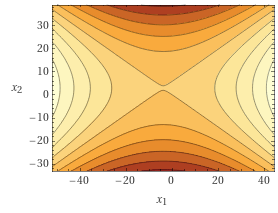
\includegraphics[width=0.8\linewidth]{part2_1c.PNG}
\caption{Contour lines of f}
\end{figure}


\textbf{2.2} \\

a. \\

\begin{align*}
f(x) = 100(x_2-x_1^2)^2+(1-x_1)^2
=
100(x_2^2 - 2x_1^2 x_2 +x_1^4)+1-2x_1 + x_1^2
= \\
100x_2^2 - 200x_1^2 x_2 +100x_1^4+1-2x_1 + x_1^2
= \\
100x_1^4+x_1^2-200x_1^2x_2-2x_1+100x_2^2+1
\end{align*} \\

\begin{align*}
\frac{\partial f }{\partial x_1} = 400x_1^3+2x_1-400x_1x_2 - 2 \\
\frac{\partial f }{\partial x_2} = -200x_1^2+200x_2
\end{align*} \\

To find a stationary point, we'll compare the derivative of f to 0 and extract $x_1,x_2$: \\

\begin{align*}
0=\nabla f= \begin{pmatrix} \frac{\partial f }{\partial x_1} \\ 
							\frac{\partial f }{\partial x_2}
			\end{pmatrix}
\end{align*} \\

\begin{tabular}{ccc}
$400x_1^3+2x_1-400x_1x_2 - 2=0$ &  \\
$-200x_1^2+200x_2=0$ & \\
\end{tabular} \\

From the second line we get that $x_2=x_1^2$, so: \\

$0=400x_1^3+2x_1-400x_1^3 - 2 \rightarrow x_1=1, \; x_2=1^2=1$\\

Now let's calculate the second derivatives to calculate the determinant of the Hessian: \\

\begin{align*}
\frac{\partial ^2 f}{\partial x_1^2}
=
\frac{400x_1^3+2x_1-400x_1x_2 - 2}{\partial x_1}
=
1200x_1^2-400x_2+2 \\
\frac{\partial ^2 f}{\partial x_2^2} = \frac{-200x_1^2+200x_2}{\partial x_2} =200 \\
\frac{\partial f}{\partial (x_1 x_2)} = \frac{-200x_1^2+200x_2}{\partial x_1}=-400x_1 \\ \\
\nabla^2f(x) = \begin{pmatrix}
1200x_1^2-400x_2+2 & -400x_1 \\
-400x_1            & 200
 \end{pmatrix}
\end{align*} \\

b. \\

The determinant of the Hessian in the point that we found (1,1): \\
\begin{align*}
\begin{vmatrix} 1200-400+2 & -400 \\ -400 & 200 \end{vmatrix}
=
\begin{vmatrix} 802 & -400 \\ -400 & 200 \end{vmatrix}
=
802 \cdot 200 - (-400)\cdot(-400) = 400 >0
\end{align*} \\

Since the determinant of the Hessian is positive and so is $\frac{\partial^2 f}{\partial x_1^2}$ - the point is a local minimum. \\

\newpage\underline{\textbf{Part 3}}:\\
\textbf{3.1} \\

Let $C_1,...,C_n$ be convex sets and x,y be points in their intersection ($x,y \in \bigcap_{i \in \{1,...n\}} C_i$).
Since x,y are points in the intersection, they're points in each of the sets $C_1,...,C_n$. Hence the line segment x-y is in each of $C_1,...,C_n$ (by virtue of each one of them being convex) and hence the line segment x-y is, by definition, in the intersection of $\bigcap_{i \in \{1,...n\}} C_i$. \\
Since this is true for every x,y that are in the intersection - the intersection $\bigcap_{i \in \{1,...n\}} C_i$ is convex. Q.E.D \\

\textbf{3.2} \\

Let $C_1,...,C_n$ be convex sets and x,y be points in their sum ($x,y \in \sum_{i=1}^{n} C_i$). x,y are themselves sums of members of $C_i$, i.e. $x = \sum_{i=1}^n x_i, \; y = \sum_{i=1}^n y_i, \;\; x_i, y_i \in C_i$. \\

We can see that for $i \; (1 \leq i \leq n)$, since $C_i$ is convex, we get: $tx_i+(1-t)y_i \in C_i \; (t\in [0,1])$. And so we get for $t\in [0,1]$: \\
\begin{align*} \\
tx_i+(1-t)y_i \in C_i \implies \sum_{i=1}^n \left( tx_i+(1-t)y_i \right)
\in \sum_{i=1}^n C_i \implies \\
t \sum_{i=1}^n x_i + (1-t) \sum_{i=1}^n y_i \in \sum_{i=1}^n C_i \implies
tx + (1-t)y \in \sum_{i=1}^n C_i
\end{align*} \\

Since we got $tx + (1-t)y \in \sum_{i=1}^n C_i \; (t\in[0,1])$ we can say that $ \sum_{i=1}^n C_i$ is convex. Q.E.D\\


\textbf{3.3} \\
Let X be a convex set and let Y be an affine transformation of X. In addition. let $y_1,y_2 \in Y$. That means that there exists $x_1,x_2 \in X$ s.t. $y_1 = Ax_1+b, \; y_2 = Ax_2 +b$. Since X is convex, we can say that $tx_1 + (1-t)x_2 \in X \;(t \in [0,1])$. Let's mark that with c:\\
$c=tx_1 + (1-t)x_2 \in X \;(t \in [0,1])$\\

Since c is in X, we can look a d that's defined as: d=Ac+b and see that $d \in Y$.
Let's break down d:\\
$d = Ac+b = A(tx_1 + (1-t)x_2)+b = tAx_1 + (1-t)Ax_2+b$.\\

Of course that $b = tb +(1-t)b$, so we get: \\

$d = tAx_1 + (1-t)Ax_2+b = tAx_1 + (1-t)Ax_2+tb +(1-t)b = t(Ax_1+b)+(1-t)(Ax_2+b) = 
ty_1+(1-t)y_2, \; (t\in[0,1])$.\\

Since $y_1,y_2 \in Y$ we get that Y in convex. Q.E.D\\

\textbf{3.4} \\

The answer is yes for a closed ball and no for an open one. Proof:\\

Let B be a ball of radius r ($r \in \mathbb{R}^+$) around an origin s.t. $B=\{ x : \|x\| \leq r \}$. Let $x,y \in B$ (so $\|x\| \leq r$, $\|y\| \leq r$).\\

Let's define a new vector and by showing that's in B as well we'll conclude that B is convex.\\

Define $z=tx+(1-t)y, \; t \in [0,1]$. Let's look at the norm of z:\\

$\|z\| \stackrel{(i)}{=} \|tx+(1-t)y\| \stackrel{(ii)}{\leq}  \|tx\|+\|(1-t)y\| \stackrel{(iii)}{=} t\|x\|+(1-t)\|y\| \stackrel{(iv)}{\leq} tr+(1-t)r = r$\\
$\implies \|z\| \leq r \implies z \in B \implies$ B in convex. Q.E.D\\

Explanations:\\
(i)   Definition of z\\
(ii)  Properties of norm\\
(iii) Properties of norm\\
(iv)  As aforementioned, $\|x\| \leq r$, $\|y\| \leq r$\\

This won't hold for a closed ball since the inequality in (ii) will still be weak and we won't be able to prove a strict inequality. \\

\textbf{3.5} \\

Let's look at the set $G = \{ x : Ax \leq b \wedge Cx = d\}$ - which is the set of solutions for some set of linear equalities and inequalities.

Let's look at $x,y \in G$, we know that $Ax \leq b, \; Cx=d, \; Ay \leq b, \; Cy=d$.\\
Let $t\in [0,1]$ and z=tx+(1-t)y. \\
$Az = tAx+(1-t)Ay \leq tb+(1-t)b = b$ \\
Cz = tCx +(1-t)Cy = td +(1-t)t = d \\

Combining the two we get that $Az \leq b \wedge Cz=d \implies $ G is convex. Q.E.D \\

\textbf{3.6} \\
Let $f,g,\alpha,\beta$ as defined in the question and a function: $h(x)=\alpha f(x) + \beta g(x)$.\\

from the definition of a convex function, if we want to prove that h is a convex function, suffice it to show that $\forall t\in [0,1], x,y$ it holds that $h(tx+(1-t)y) \leq th(x)+(1-t)h(y)$. Let's show exactly that:\\

\begin{align*} \\
h(tx+(1-t)y) = \alpha f(tx+(1-t)y) +\beta g(tx+(1-t)y) \stackrel{(since \; f,g \; are \; convex)}{\leq} \\
\alpha (t f(x)+(1-t)f(y)) + \beta tg(x)+(1-t)g(y)) = \\
t(\alpha f(x) + \beta g(x)) + (1-t)(\alpha f(y) + \beta g(y)) =\\
th(x)+(1-t)h(y)
\end{align*} \\
Q.E.D\\

\textbf{3.7} \\

The proof will be very similar to the previous section: \\
Let f,g be convex function and h their pointwise max (h(x)=max{f(x),g(x)}).
Let $t \in [0,1]$:\\

\begin{align*} \\
h(tx+(1-t)y) = max\{ f(tx+(1-t)y), g(tx+(1-t)y)\} \leq \\
max\{t f(x)+(1-t)f(y), t g(x)+(1-t)g(y) \}  \leq \\
max\{t f(x), t g(x) \} + max\{(1-t) f(y), (1-t) g(y) \}  = \\
t \cdot max\{f(x), g(x) \} + (1-t)\cdot max\{f(y), g(y) \} = t \cdot h(x)+ (1-t) h(y)
\end{align*} \\
Q.E.D \\


\textbf{3.8} \\
Let $f:D \subset \mathbb{R}^n \rightarrow \mathbb{R}$ be a convex function and $A= \{ x \in D:f(x) \leq c\}$ be a sub-level set of f (where c is a constant scalar). \\
Let $x,y \in A$ and $z = tx +(1-t)y, \; t\in [0,1]$\\

Suffice it to show that $z \in A$ to conclude that A is convex. Let's do exactly that:\\

\begin{align*} \\
f(z) = f(tx +(1-t)y) \stackrel{(f \; is \; convex)}{\leq} tf(x)+(1-t)f(y) 
\stackrel{(x,y \; are \; in \; A)}{\leq}tc+(1-t)c = c \\
\implies f(z) \leq c \implies z \in A
\end{align*} \\

Q.E.D \\


\textbf{3.9} \\

Let f,h be as defined in the question (before the counter examples). Let's define g(x)=h(f(x)) and let $t\in [0,1]$: \\

\begin{align*} \\
g(tx+(1-t)y) = h(f(tx+(1-t)y)) \stackrel{(i)}{\leq} h(tf(x)+(1-t)f(y)) \stackrel{(ii)}{\leq}  \\ th(f(x))+(1-t)h(f(y)) = tg(x)+(1-t)g(y)
\end{align*} \\
Q.E.D \\

In (i) we used the fact that f is convex and that h is monotonic increasing. \\

In (ii) we used the fact that h is convex.\\

from those the counter examples are pretty simple ti deduce: \\

If we drop the monotonic requirements (e.g. h(x) = -3x) then (i) doesn't hold anymore (as a larger value of f(x) will result in a \textbf{lower} value of h(x)). \\

As for the convexity of h, if we drop it (e.g. $h(x)=3x^3$) than (ii) doesn't hold. \\
\end{document}\\